% Name: Waterfall chart
% Description: A profit bridge from revenue to net profit: each cost hangs down from the running total, with dashed connectors and a value on every bar.
% Tags: waterfall chart, bridge chart, profit, finance

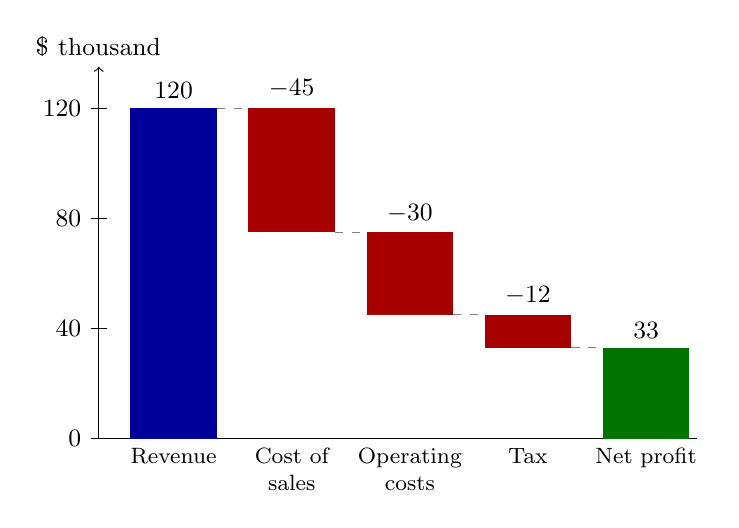
\begin{tikzpicture}[font=\small, y=0.035cm]
  % In thousands: 120 - 45 - 30 - 12 = 33; the bar for each cost spans the running total before and after it.
  \draw[->] (0,0) -- (0,135) node[above] {\$ thousand};
  \foreach \y in {0,40,80,120} \draw (0.1,\y) -- (-0.1,\y) node[left] {\y};
  \draw (0,0) -- (7.6,0);
  \fill[blue!60!black] (0.4,0) rectangle (1.5,120);
  \fill[red!65!black] (1.9,75) rectangle (3.0,120);
  \fill[red!65!black] (3.4,45) rectangle (4.5,75);
  \fill[red!65!black] (4.9,33) rectangle (6.0,45);
  \fill[green!45!black] (6.4,0) rectangle (7.5,33);
  \draw[gray, dashed] (1.5,120) -- (1.9,120) (3.0,75) -- (3.4,75) (4.5,45) -- (4.9,45) (6.0,33) -- (6.4,33);
  \foreach \x/\y/\v in {0.95/120/120, 2.45/120/$-45$, 3.95/75/$-30$, 5.45/45/$-12$, 6.95/33/33}
    \node[above] at (\x,\y) {\v};
  \foreach \x/\name in {0.95/Revenue, 2.45/Cost of sales, 3.95/Operating costs, 5.45/Tax, 6.95/Net profit}
    \node[below, align=center, text width=1.4cm, font=\footnotesize] at (\x,0) {\name};
\end{tikzpicture}
